\documentclass{beamer} 
\usetheme{Berlin}
\usepackage{showexpl} 
\usepackage{tikz}
\usepackage{chemfig}
\usepackage[utf8]{inputenc}

\usepackage{circuitikz}
\usepackage[english]{babel}
\usepackage{blindtext}
\usepackage{multicol}
\usepackage{ragged2e}



\title{Latex}
\subtitle{Applications of Derivatives}



\lstloadlanguages{[LaTeX]Tex} 
\lstset{% 
     basicstyle=\ttfamily\small, 
     commentstyle=\itshape\ttfamily\small, 
     showspaces=false, 
     showstringspaces=false, 
     breaklines=true, 
     breakautoindent=true, 
     captionpos=t 
} 
\begin{document} 


\frame {
		\titlepage
	}




%%%%%%%%%%%%%%%%%%%%%%%%%%%%%%%%%%%%%%%%%%%

\frame
{
\frametitle{Maxima Minima} 

\textbf{Question :} The slant height of a right circular cone is 3 cm. Find the height of cone, if its volume is the greatest.\\
%----------------------------------------
\vspace{0.4cm}
\textbf{Solution :} Let r  and x  be the base-radius and the height of the cone respectively. Then volume of the cone f(x) is given by

\begin{equation} \nonumber
\begin{alignedat}{4}
f(x) &= \frac{1}{3}\pi r^2x\\
&= \frac{\pi}{3}(3^2-x^2)x\\
&= \frac{\pi}{3}(9x - x^3)\\
\therefore f'(x) &=  \frac{\pi}{3}(9 - 3x^2)\\
\end{alignedat}
%\vrule
\quad\quad\quad
\begin{alignedat}{4}
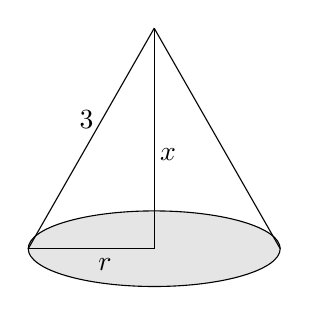
\begin{tikzpicture}[scale=0.8]
\filldraw[fill=gray!20](0,0) ellipse (2cm and 0.6cm);
\draw (0,0) -- node[below] {\ \ \ $x$}(0,3.5);
\draw (0,0)  -- node[below] {\ \ \ $r$} (-2,0);
\draw  (-2,0) --node[above] {3\ \ }(0,3.5);
\draw  (2,0) -- (0,3.5);
\end{tikzpicture}\\\\
\end{alignedat}
\end{equation}
}

%%%%%%%%%%%%%%%%%%%%%%%%%%%%%%%%%%%%%%%%%%%%

\frame
{
\frametitle{Maxima Minima} 

\textbf{Question :} The slant height of a right circular cone is 3 cm. Find the height of cone, if its volume is the greatest.\\
%----------------------------------------
\vspace{0.4cm}
\textbf{Solution :} Let r  and x  be the base-radius and the height of the cone respectively. Then volume of the cone f(x) is given by

\begin{equation} \nonumber
\begin{alignedat}{4}
f(x) &= \frac{1}{3}\pi r^2x\\
&= \frac{\pi}{3}(3^2-x^2)x\\
&= \frac{\pi}{3}(9x - x^3)\\
\therefore f'(x) &=  \frac{\pi}{3}(9 - 3x^2)\\
\end{alignedat}
%\vrule
\quad\quad\quad
\begin{alignedat}{4}
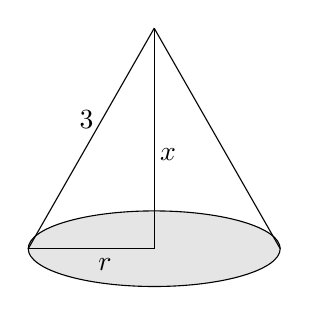
\begin{tikzpicture}[scale=0.8]
\filldraw[fill=gray!20](0,0) ellipse (2cm and 0.6cm);
\draw (0,0) -- node[below] {\ \ \ $x$}(0,3.5);
\draw (0,0)  -- node[below] {\ \ \ $r$} (-2,0);
\draw  (-2,0) --node[above] {3\ \ }(0,3.5);
\draw  (2,0) -- (0,3.5);
\end{tikzpicture}\\\\
\end{alignedat}
\end{equation}
}

%%%%%%%%%%%%%%%%%%%%%%%%%%%%%%%%%%%%%%%%%%%%





\end{document}